\documentclass[11pt, a4paper]{article}
\usepackage[utf8]{inputenc}
\usepackage[spanish]{babel}
\usepackage{graphicx}
\usepackage{float}
\usepackage{geometry}
\geometry{a4paper, margin=2.5cm}
\usepackage{hyperref}

\title{Informe de Métricas de Nodos SDR: ANE6, ANE7 y ANE8}
\author{David Ramírez Betancourth}
\date{\today}

\begin{document}

\maketitle

\section{Introducción}
Este documento presenta la recopilación y análisis de métricas de hardware y red para tres nodos de monitoreo basados en Raspberry Pi 5 (ANE6, ANE7, ANE8). Las métricas analizadas incluyen la tensión del riel de 5V (\texttt{EXT5V\_V}), la temperatura del núcleo ARM (\texttt{temp}) y la pérdida de paquetes en la interfaz LTE ppp0 (\texttt{packet\_loss}).

\section{Métricas Nodo ANE6}

\begin{figure}[H]
    \centering
    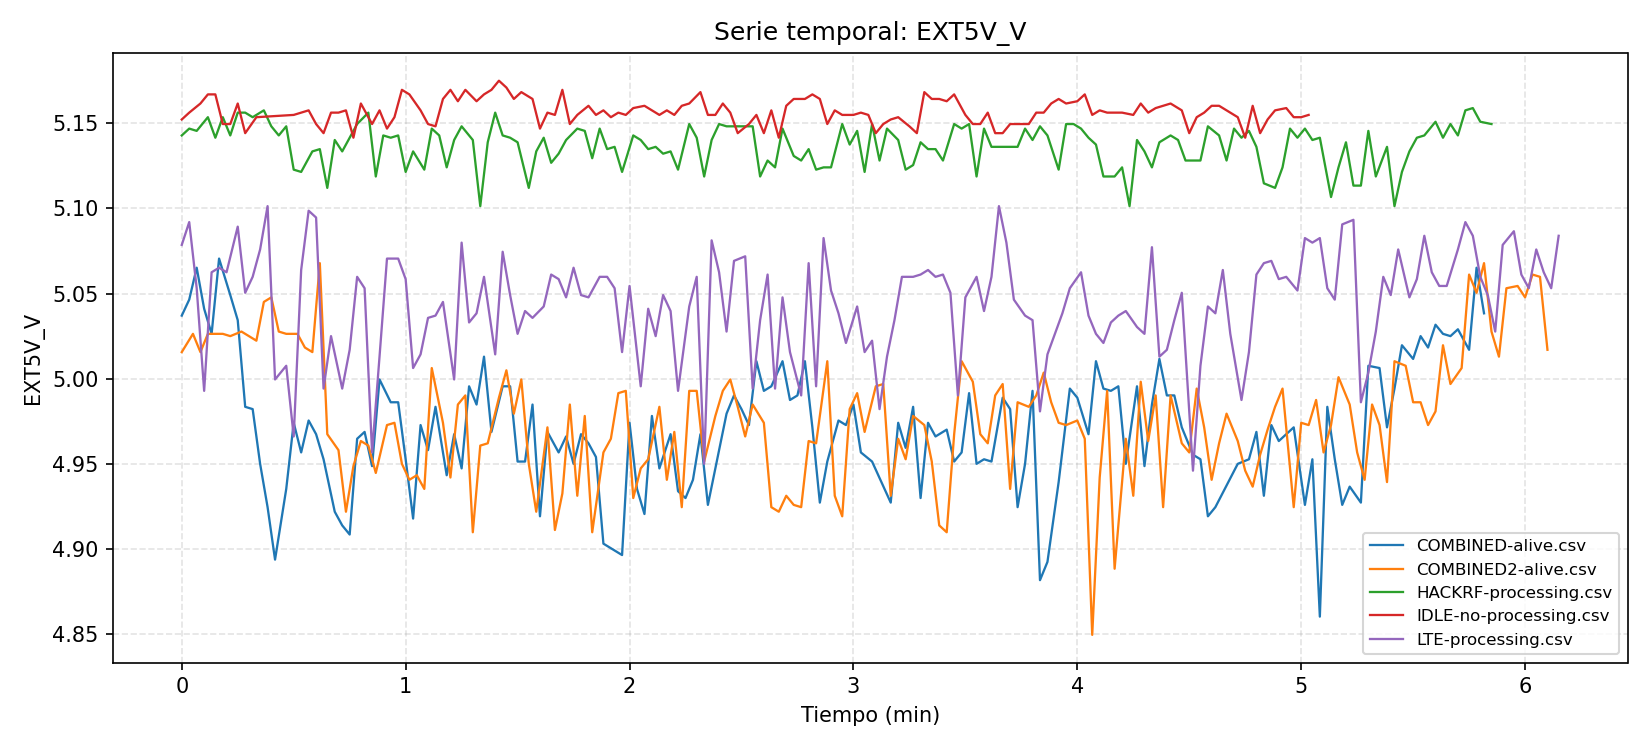
\includegraphics[width=0.8\textwidth]{ANE6-EXT5V_V.png}
    \caption{Serie temporal de tensión EXT5V\_V - Nodo ANE6.}
\end{figure}

\begin{figure}[H]
    \centering
    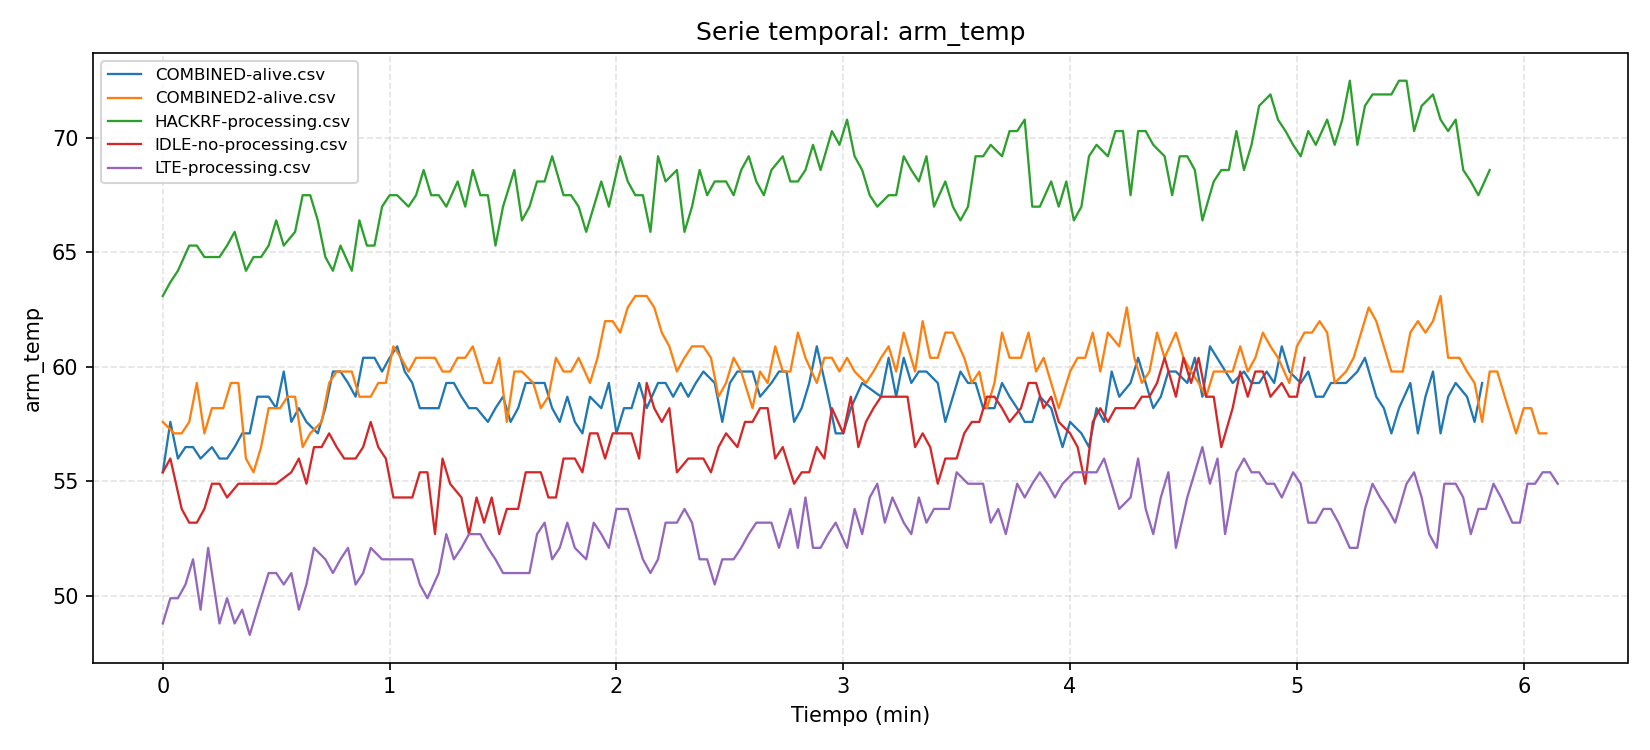
\includegraphics[width=0.8\textwidth]{ANE6-temp.png}
    \caption{Serie temporal de temperatura del ARM - Nodo ANE6.}
\end{figure}

\begin{figure}[H]
    \centering
    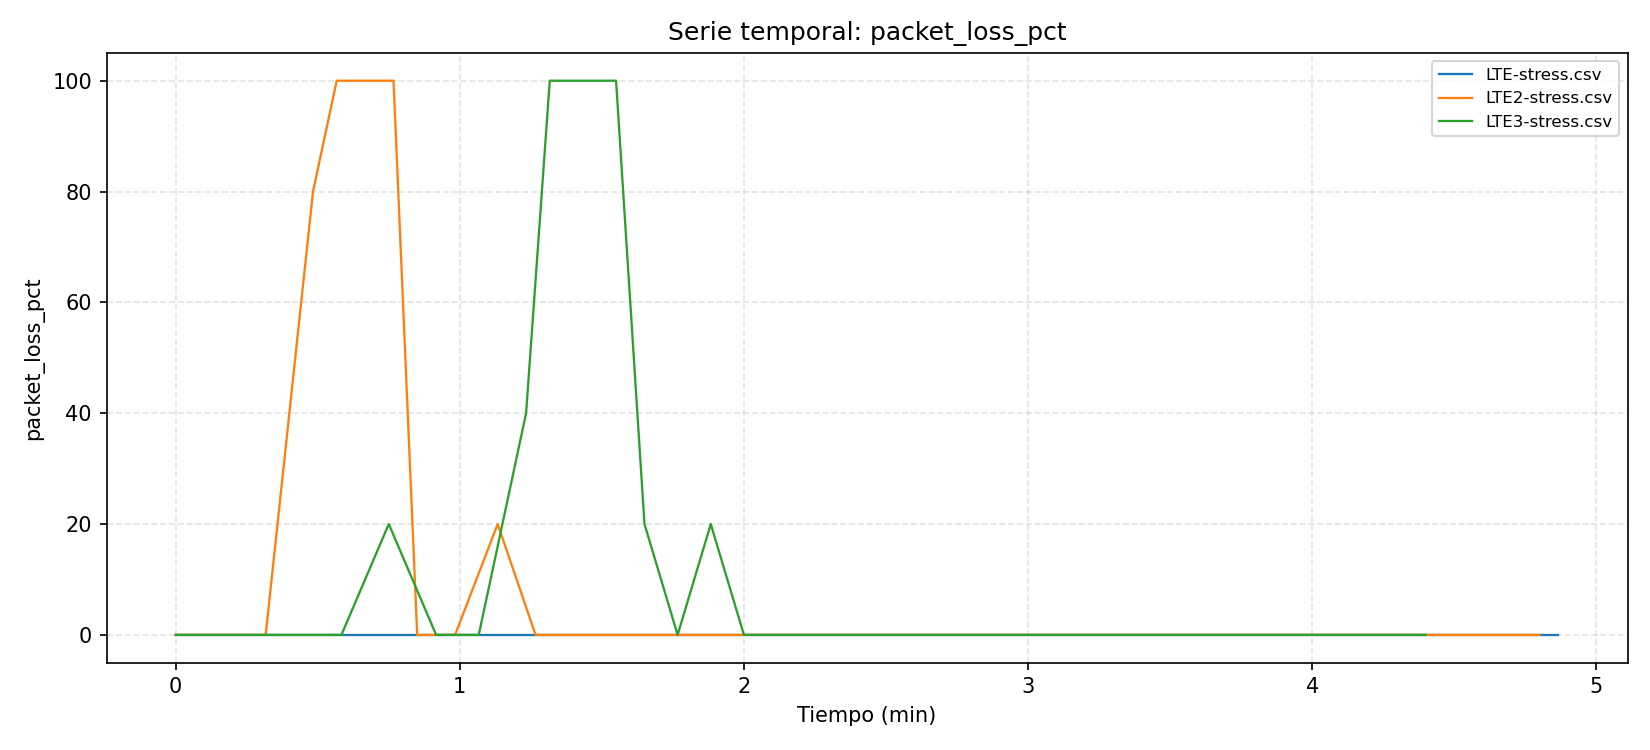
\includegraphics[width=0.8\textwidth]{ANE6-packet-loss.png}
    \caption{Serie temporal de pérdida de paquetes LTE - Nodo ANE6.}
\end{figure}


\section{Métricas Nodo ANE7}

\begin{figure}[H]
    \centering
    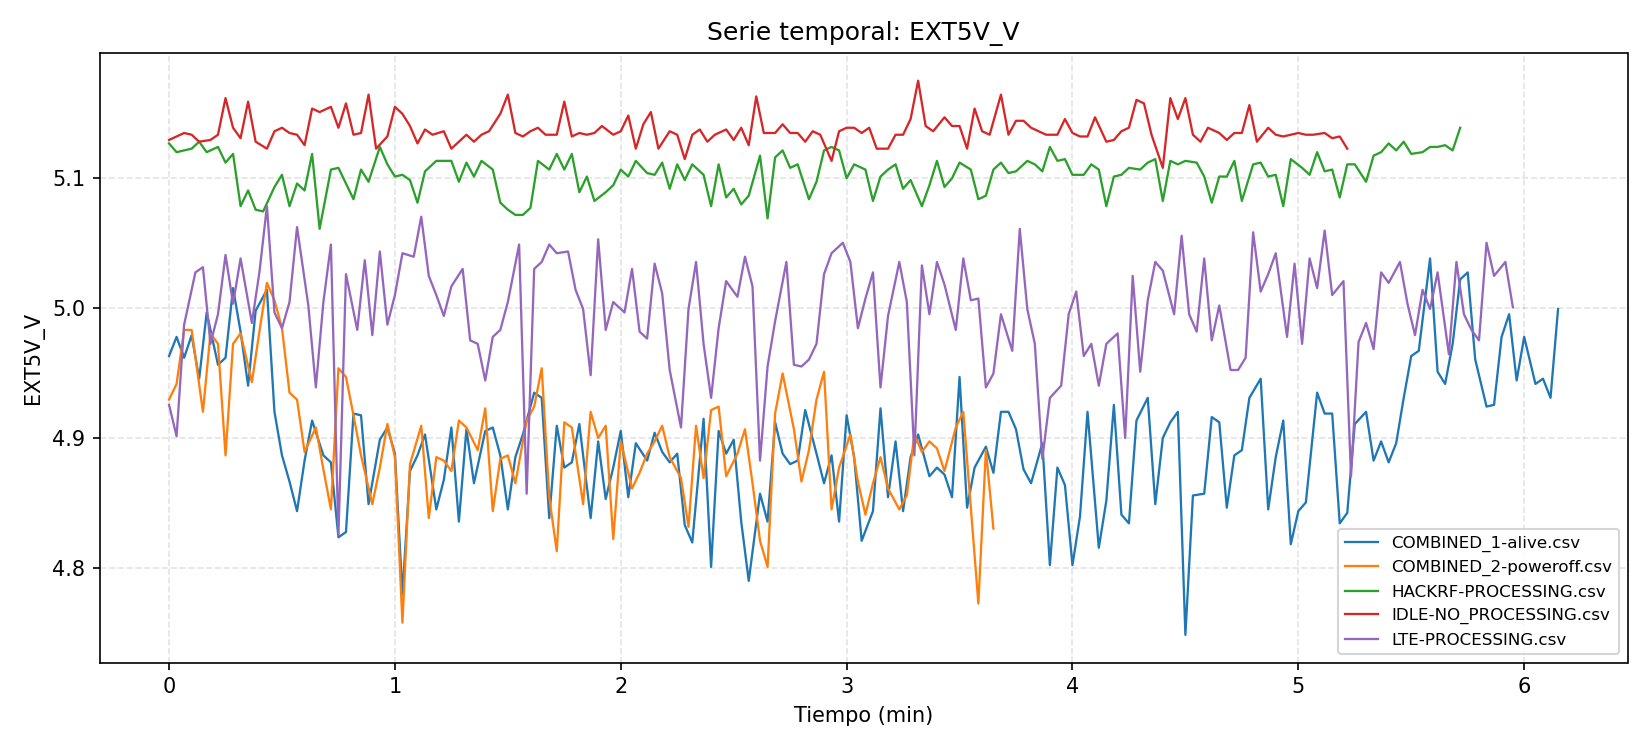
\includegraphics[width=0.8\textwidth]{ANE7-EXT5V_V.png}
    \caption{Serie temporal de tensión EXT5V\_V - Nodo ANE7.}
\end{figure}

\begin{figure}[H]
    \centering
    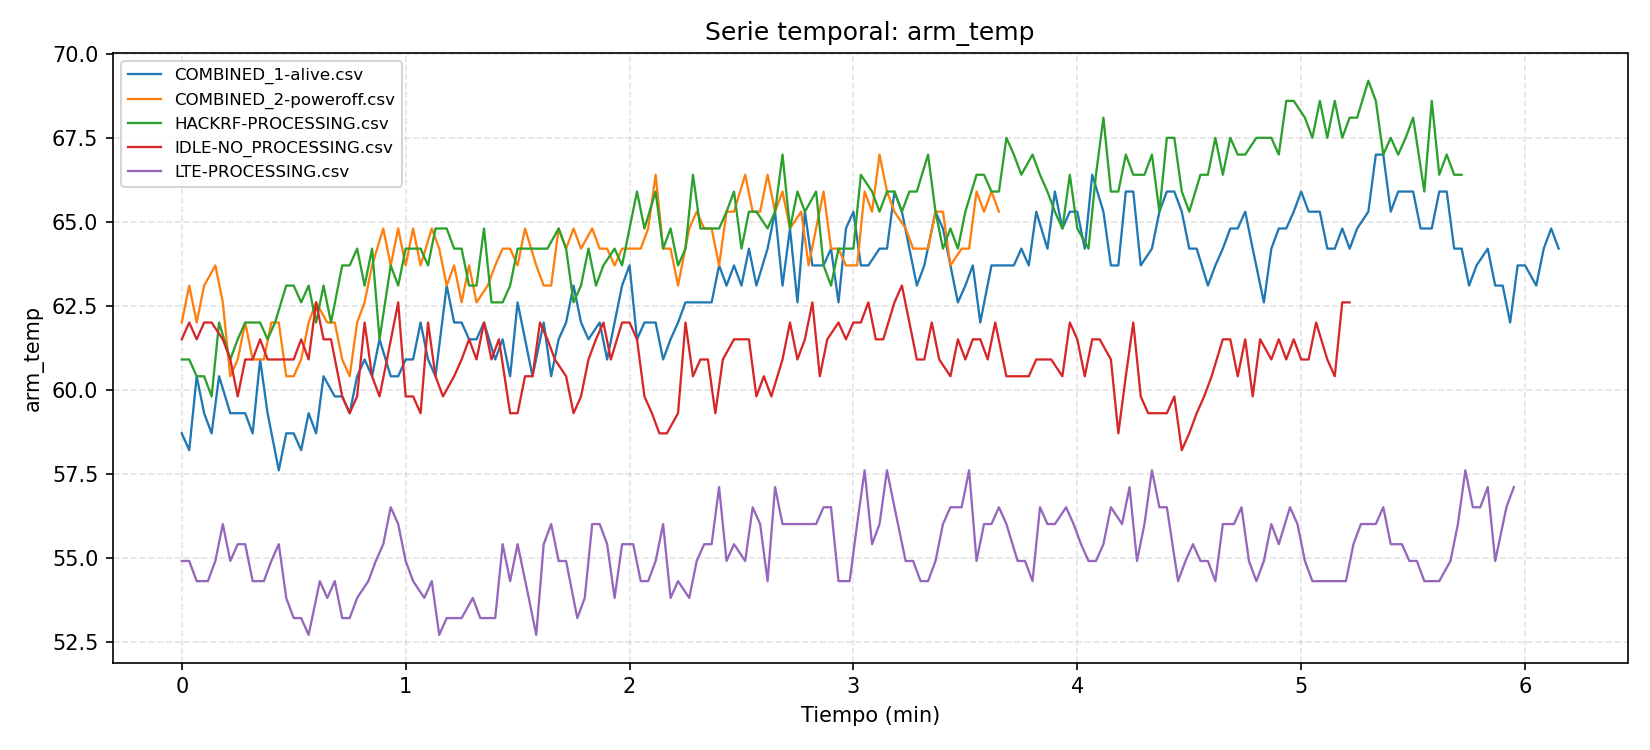
\includegraphics[width=0.8\textwidth]{ANE7-temp.png}
    \caption{Serie temporal de temperatura del ARM - Nodo ANE7.}
\end{figure}

\begin{figure}[H]
    \centering
    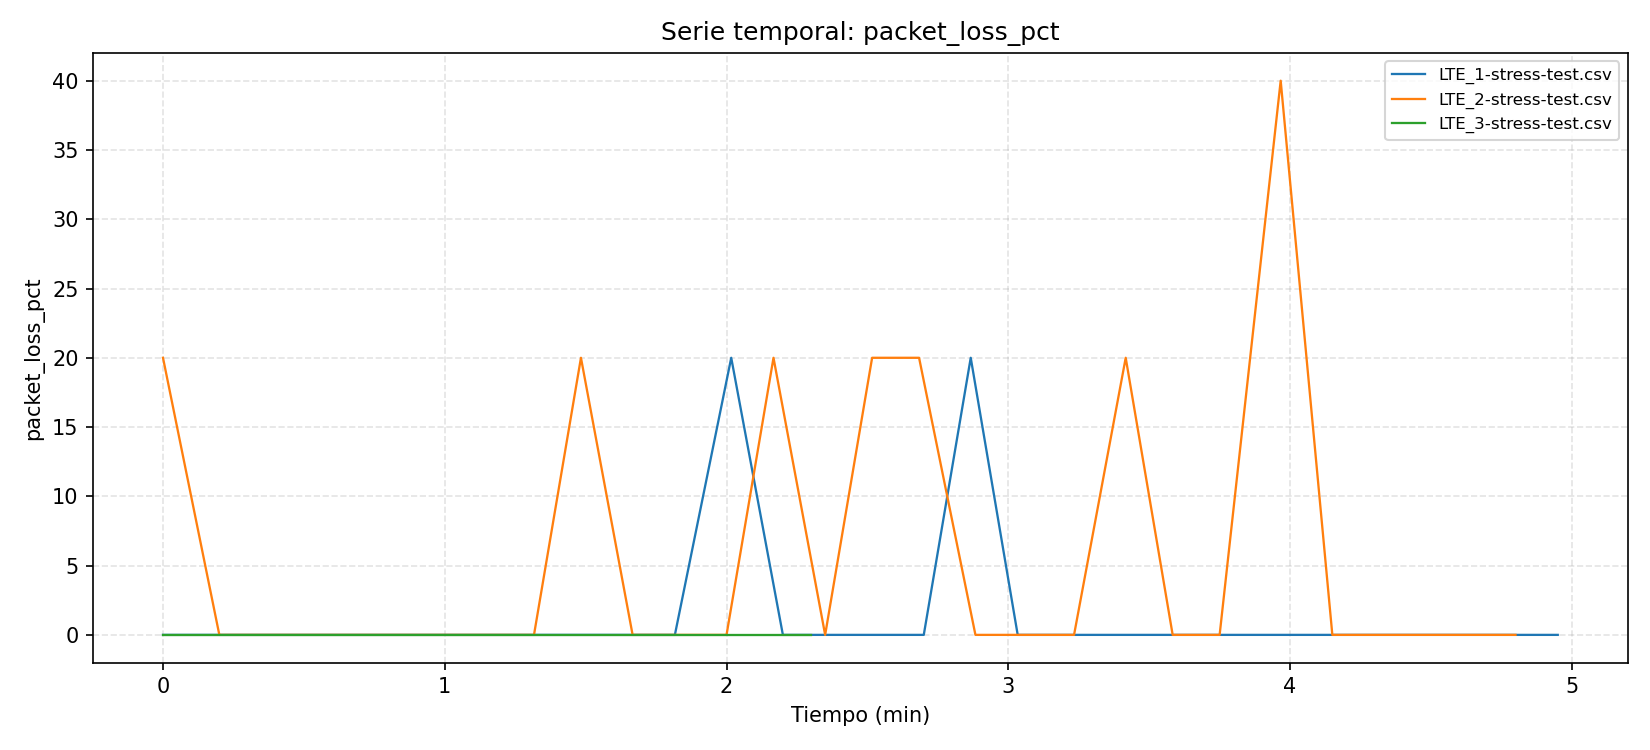
\includegraphics[width=0.8\textwidth]{ANE7-packet-loss.png}
    \caption{Serie temporal de pérdida de paquetes LTE - Nodo ANE7.}
\end{figure}


\section{Métricas Nodo ANE8}

\begin{figure}[H]
    \centering
    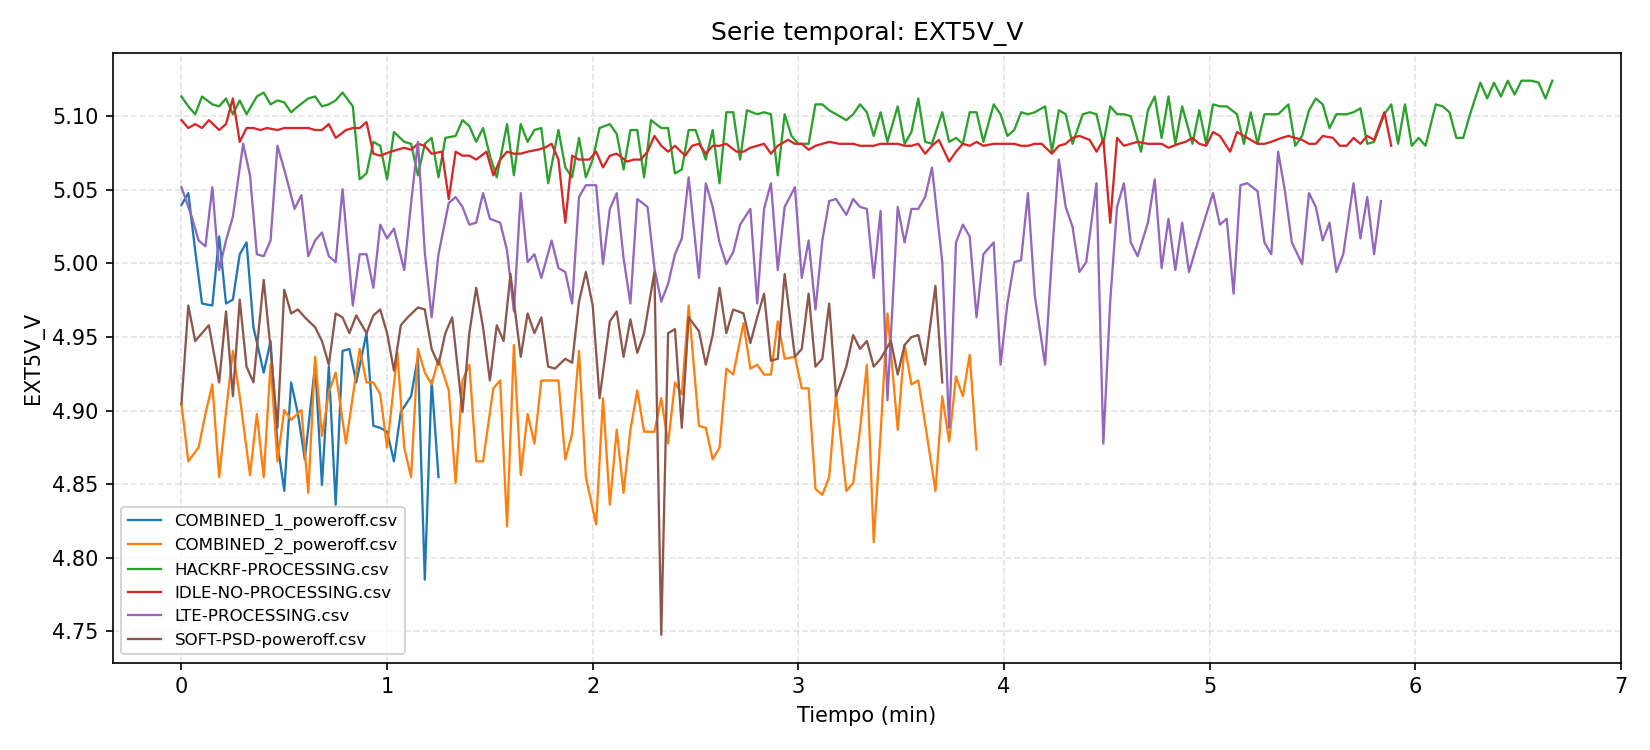
\includegraphics[width=0.8\textwidth]{ANE8-EXT5V_V.png}
    \caption{Serie temporal de tensión EXT5V\_V - Nodo ANE8.}
\end{figure}

\begin{figure}[H]
    \centering
    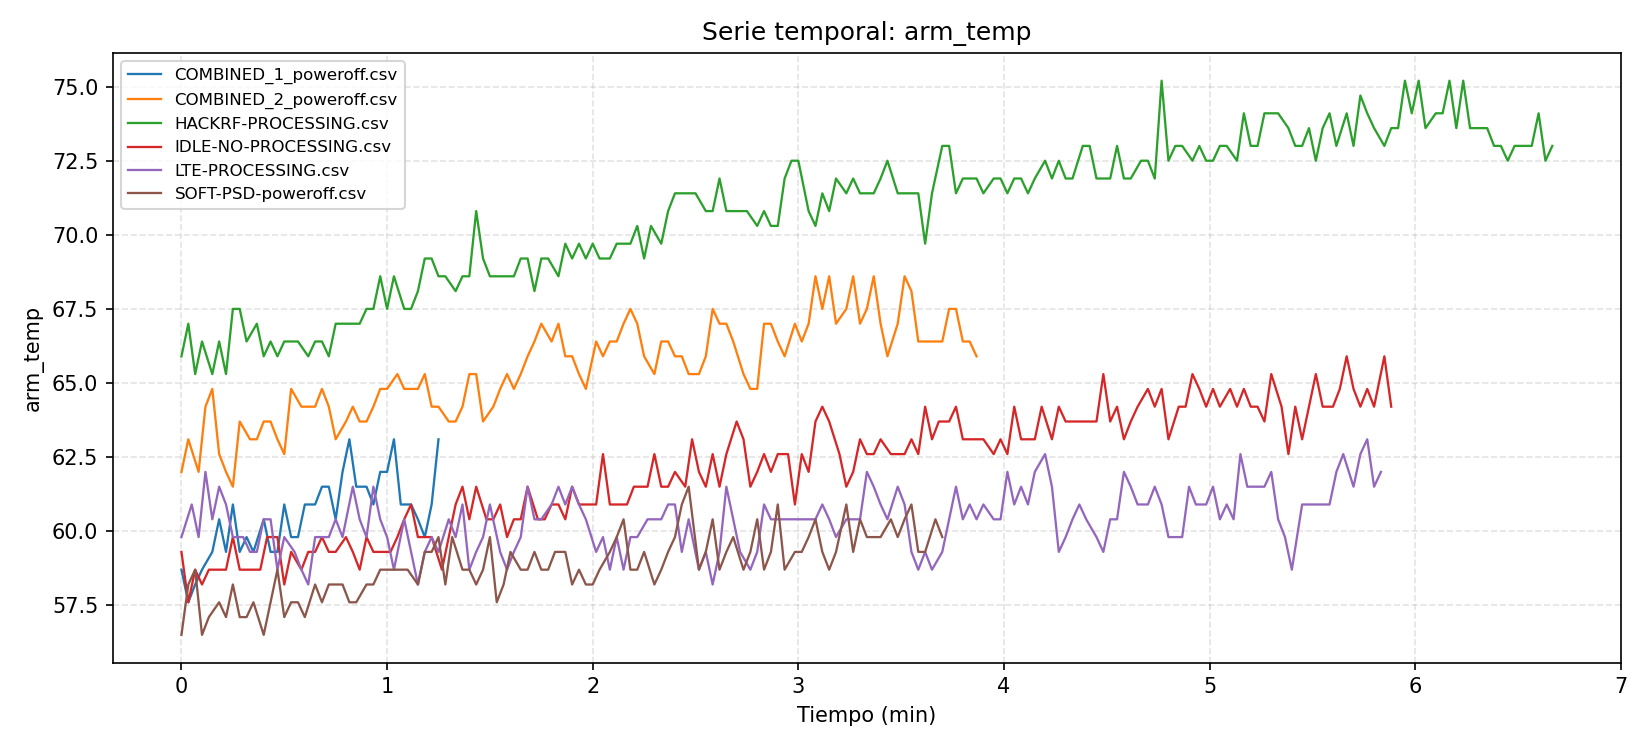
\includegraphics[width=0.8\textwidth]{ANE8-temp.png}
    \caption{Serie temporal de temperatura del ARM - Nodo ANE8.}
\end{figure}

\begin{figure}[H]
    \centering
    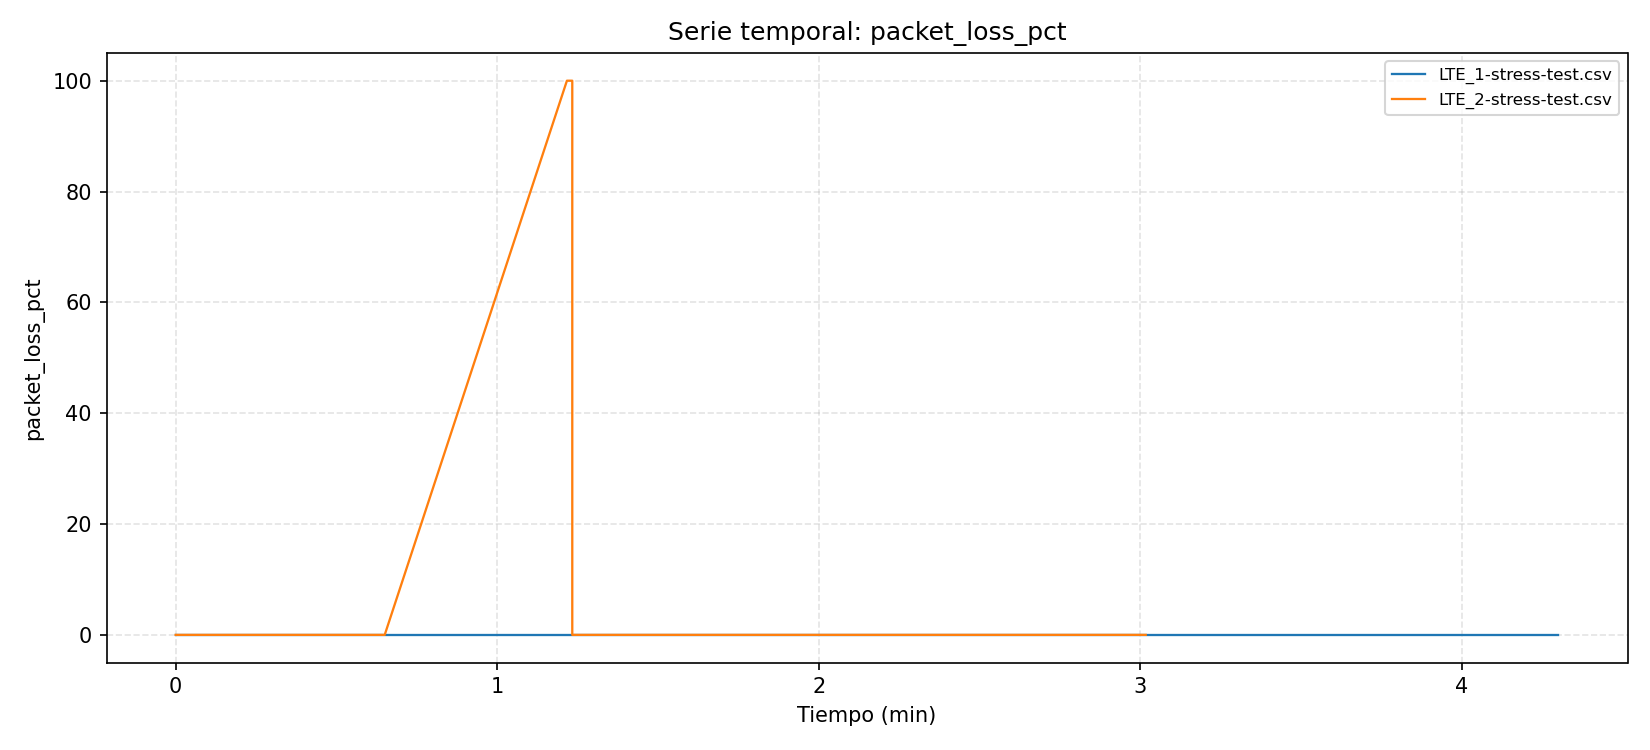
\includegraphics[width=0.8\textwidth]{ANE8-packet-loss.png}
    \caption{Serie temporal de pérdida de paquetes LTE - Nodo ANE8.}
\end{figure}


\section{Análisis Técnico}

Con base en la telemetría extraída de los tres nodos de sensor, se identifican los siguientes comportamientos sistémicos bajo diferentes perfiles de carga:

\subsection{Integridad de Potencia (EXT5V\_V)}
Se observa una caída de tensión (\textit{voltage droop}) significativa en el riel \texttt{EXT5V\_V} durante los perfiles de estrés combinado (\texttt{COMBINED}), descendiendo desde un estado de reposo estable de $\approx 5.15\text{V}$ hasta valores de $4.80\text{V} - 4.75\text{V}$ (particularmente en ANE7 y ANE8). Estas fluctuaciones en régimen transitorio indican que la fuente de alimentación está operando cerca de su límite de regulación cuando concurren el estrés del CPU, la alimentación USB del HackRF y los picos de transmisión del módulo LTE, siendo la caída más significativa de voltaje al usar el LTE. Caídas por debajo de $4.8\text{V}$ pueden inducir \textit{brownouts} o reinicios en el módem celular o en el front-end de RF.

\subsection{Estabilidad de Red (Packet Loss)}
Las pruebas de estrés sobre la interfaz \texttt{ppp0} (\texttt{LTE-stress}) revelan un problema crítico de fiabilidad en el enlace. Se registran picos de pérdida de paquetes de hasta el $100\%$ en ráfagas para los nodos ANE6 y ANE8, y variaciones de $20\%-40\%$ en ANE7. Esta alta tasa de pérdida coincide temporalmente con las pruebas de máxima carga, lo que sugiere una de dos hipótesis: o bien existe una saturación de colas y desbordamiento de buffers en el stack de red bajo condiciones de estrés, o las caídas de tensión previamente descritas están comprometiendo la estabilidad del procesador \textit{baseband} del módulo LTE, provocando reinicios silentes o caídas temporales del portador celular.

\end{document}